% !TEX root = MAIN.tex
\clearpage
\section{Code-driven Mutation Testing (Test Suite Augmentation)}
\label{sec:testGeneration:codeDriven}

\subsection{Overview}

We address the following research questions:

\emph{RQ1. Does SEMuS scale in the context of space software?}

\emph{RQ2. Does SEMuS improve the mutation score of test suites?}

\subsection{Subjects of the Study}

\TODO{add subjects of the study: Libutil + ESAIL Unit TS}

To perform our experiments, we considered two software artifacts, both of them provided by the European Space Agency (ESA): ASN1SCC (or ASN.1) and MLFS.
In the case of ASN.1, the test suite is automatically generated with an approach that aims to maximize the boundary conditions of the input domain being covered. 
The Mathematical Library for Flight Software (MLFS) implements mathematical functions qualified for flight software (it complies with ECSS criticality category B).
Both test suites considered in this study characterize by high statement coverage as required by space software standards (e.g., category C software requires statement adequacy according to ECSS). MLFS test suite achieves MC/DC coverage (i.e., 100\% coverage), while ASN.1 case study achieves 99\% statement coverage.

% \TODO{to be fixed}
% \REVOCT{C-P-19}{We did not considered ESAIL in our empirical evaluation, because of the known incompatibility of clang (i.e., the compiler required by SEMuS) and ESAIL specific compilation libraries (i.e., RTEMS). More details can be found in Section~\ref{}.}

\subsection{Setup}

\TODO{Libutil: we considered four sources (clock.c, memory.c, error.c, and timestamp.c), these files make part of the set of sources that are interesting for GSL. They were also the only files for which we were capable of generating tests, the rest of sources had FILES dependencies, and functions requiring I/O operations. We considered a total of 79 mutants for clock, 22 for memory, 4 for error, and 8 timestamp. Then, we generated 2 tests for clock, 55 for memory, 16 for error, and 9 for timestamp.}
\TODO{ESAIL: we considered one source(TMFrameBuilder.c). This source was the only one with little dependencies from other components, from the set of sources selected by Yago at the beginning of the project. We used 5 mutants from two functions, already killed by both test suites. We generated a total of 9 tests for the source under test.}

To address our research questions, we consider mutation analysis a precondition for our subjects; this is necessary since test generation only requires the list of live mutants (i.e., generating test inputs for all possible mutants would be far too expensive). Table~\ref{table:results:semus:ms} reports the mutation analysis results (i.e., MASS output) for the ASN.1 and MLFS subjects.

\begin{table}[htb]
\caption{Mutation scores for artifacts.}
\label{table:results:semus:ms} 
\centering
\begin{tabular}{|
@{\hspace{1pt}}p{20mm}|
@{\hspace{1pt}}>{\raggedleft\arraybackslash}p{20mm}@{\hspace{1pt}}|
>{\raggedleft\arraybackslash}p{15mm}@{\hspace{1pt}}|
>{\raggedleft\arraybackslash}p{15mm}@{\hspace{1pt}}|
 >{\raggedleft\arraybackslash}p{35mm}@{\hspace{1pt}}|
}
\hline
\textbf{Subject}&\textbf{Mutants}&\textbf{Killed}&\textbf{Live}&\textbf{Mutation Score (\%)}\\ 
\hline
$\mathit{MLFS}$&21\,375&17\,484&3\,891&81.80 \\
$\mathit{ASN.1}$&5\,323&3\,104&2\,219&58.31 \\
$\mathit{ESAIL_S}$ (S+U)&3\,536&2\,495&1\,041&70.56 \\
$\mathit{Libutil}$&21\,375&17\,484&4\,198&81.80 \\ %35
\hline
\end{tabular}

\end{table}

As shown in Table~\ref{table:results:semus:ms}, we apply test generation for the 3\,891 live mutants of MLFS, and for the 2\,219 live mutants of the ASN.1 subject.
For every subject, we applied the SEMuS toolset on Linux OS running on the HPC cluster of the University of Luxembourg. The HPC cluster consists of Intel Xeon E5-2680 v4 (2.4 GHz) nodes. To make our experiments feasible we executed 14 SEMuS parallel instances running on a dedicated node.

\subsection{RQ1 - Approach scalability}
\label{sec:rq1:semus}

To assess \INDEX{SEMuS} scalability we measure the execution time of each SEMuS instance. Table~\ref{table:results:semus:times} shows statistics about execution times for MLFS and the ASN.1 subjects.
Firstly, we notice is that median time taken by SEMuS to generate test inputs is the same for both case studies (i.e., 0.4 minutes). While, the mean differs for both case studies, 8.5 minutes for MLFS, and 33.4 for ASN.1 case study. Secondly, we notice that the maximum execution time is limited by the configuration we imposed in SEMuS for the symbolic search, that is, two hours.
Lastly, we notice that the total execution time of MLFS is approximately 556 hours, which can be executed on only 5.5 hours if executed with 100 HPC nodes. Similarly, the ASN.1 subject can be executed in approximately 1\,161 hours, or 11.6 hours if executed with 100 HPC nodes. In this context, even paying for the computational power of 100 HPC nodes for making test generation feasible in half a day is economically justifiable in the space software context.

    \begin{figure}[tb]
    \centering
        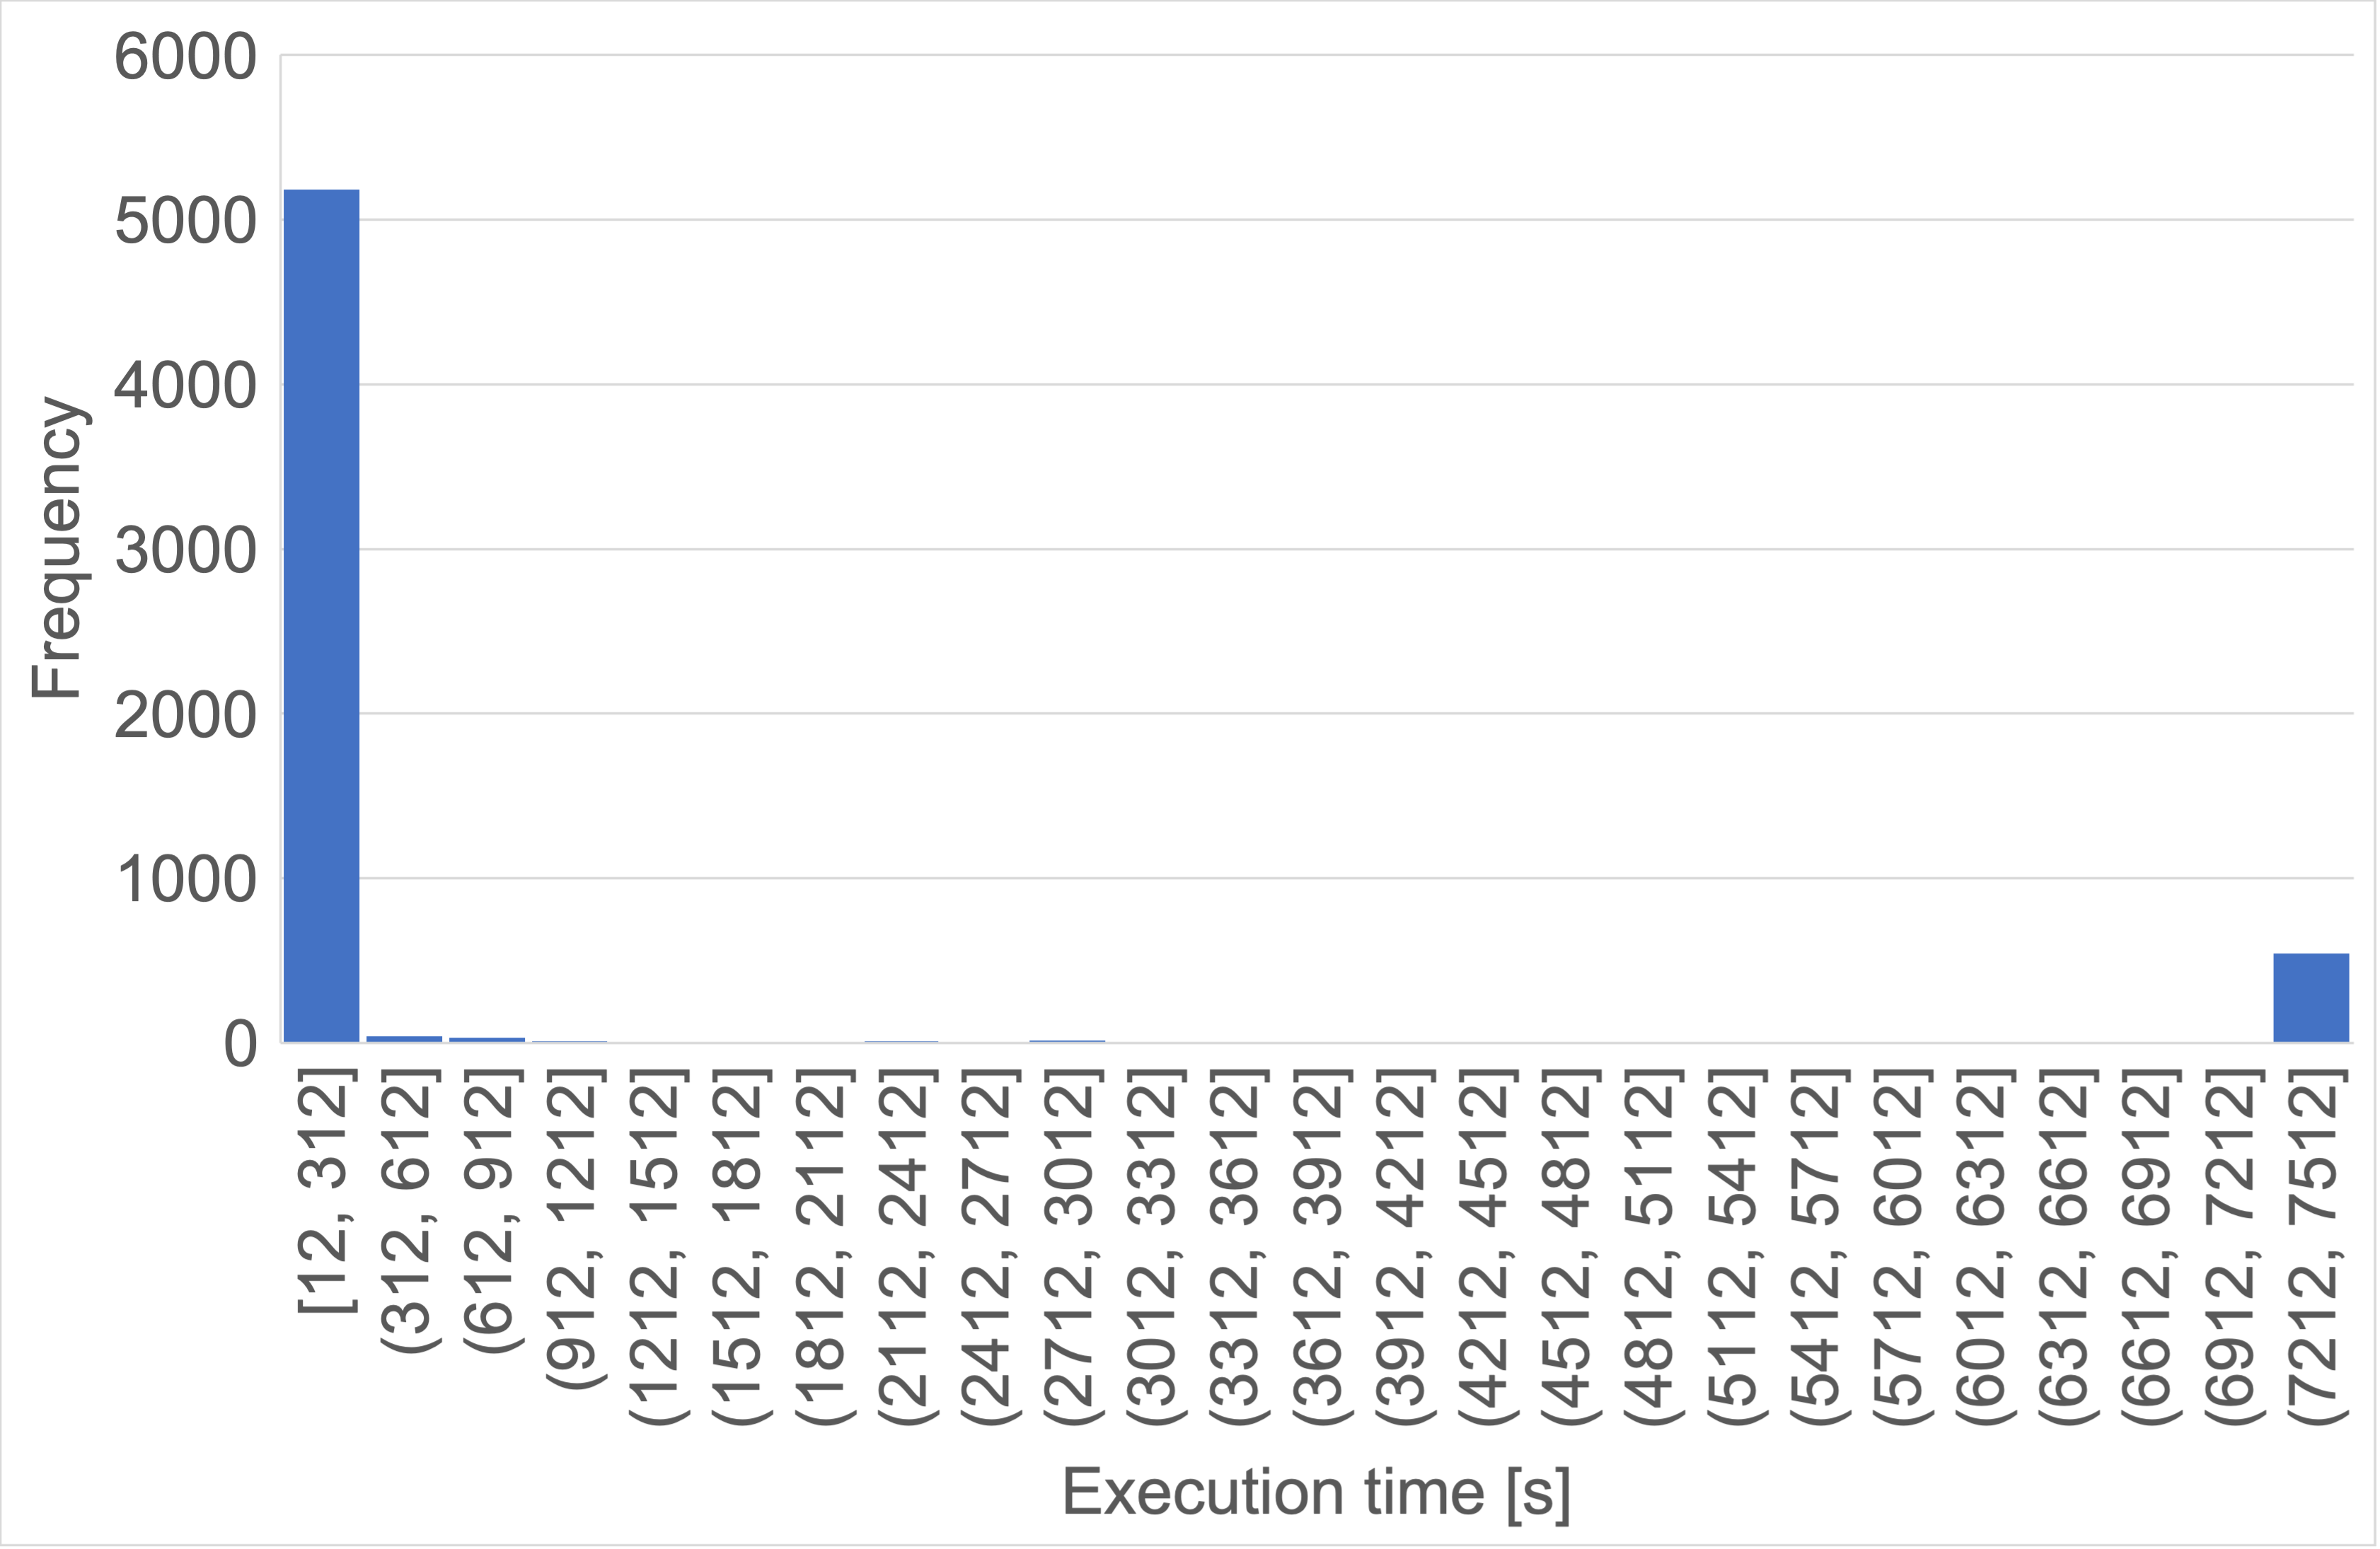
\includegraphics[width=0.7\textwidth]{images/execution_time}
        \caption{SEMuS execution time histogram.}
        \label{fig:semus:histogram_time}
    \end{figure}

\REVOCT{TDR-SUM-PABG-01}{Furthermore, we report in Figure~\ref{fig:semus:histogram_time} the histogram of the execution time of all test cases generated for both ASN.1 and MLFS. Particularly, we can see that for 5\,068 mutants (89.11\%) the test case generation time was approximately 5 minutes, and that only 545 mutants took 2 hours approximately (the maximum time configured for our experiments, which leads to test cases not being generated). In line with these results, we conclude that test generation with SEMuS scale.}


\begin{table}[htb]
\caption{SEMuS execution times.}
\label{table:results:semus:times} 
\centering
\footnotesize
\begin{tabular}{|
@{\hspace{1pt}}p{10mm}|
@{\hspace{1pt}}>{\raggedleft\arraybackslash}p{10mm}@{\hspace{1pt}}|
>{\raggedleft\arraybackslash}p{15mm}@{\hspace{1pt}}|
>{\raggedleft\arraybackslash}p{20mm}@{\hspace{1pt}}|
 >{\raggedleft\arraybackslash}p{15mm}@{\hspace{1pt}}|
 >{\raggedleft\arraybackslash}p{25mm}@{\hspace{1pt}}|
 >{\raggedleft\arraybackslash}p{15mm}@{\hspace{1pt}}|
}
\hline
\textbf{Subject}&\textbf{Min [m]}&\textbf{Max [m]}&\textbf{Median [m]}&\textbf{Mean [m]}&\textbf{Std. Deviation [m]}&\textbf{Total [m]}\\ 
\hline
$\mathit{MLFS}$&0.2&122.5&0.4&8.5&30.2&33\,348.4\\
$\mathit{ASN.1}$&0.2&121.3&0.4&33.4&54.6&69\,696.2\\
$\mathit{ESAIL_S}$&0.3&0.5&0.4&0.4&0.1&2.0\\
$\mathit{Libutil}$&0.3&0.6&0.4&0.4&0.1&41.8\\
\hline
\end{tabular}

\end{table}


\subsection{RQ2 - Approach effectiveness}


To assess the approach effectiveness, we verify whether SEMuS succeeds to generate test inputs that kills non detected mutants from our subjects. We consider SEMuS effective, if the approach improves the subject mutation score.

Table~\ref{table:results:semus:testgen} shows the variations we observed in the subjects' mutation scores, the table presents the number of live mutants, the additionally killed mutants by SEMuS, the original mutation score, and the updated mutation score.
Particularly, we observe that SEMuS kills additional 1\,729 mutants for the ASN.1 subject, increasing the mutation score from 58.31\% to 90.79\%, an impressive improvement of 32,48\%.
Instead, we observe that SEMuS kills additional 697 mutants for the MLFS subject, increasing the mutation score from 81.80\% to 85.06\%, an improvement of 3,26\%.

The lower improvement observed on the MLFS could be explained by the following reasons: (1) possible presence of many equivalent mutants, (2) bugs in SEMuS fixed recently, and (3) known limitations of KLEE (i.e., the underlying test generation tool) concerning floating-point analysis. These limitations can be assessed in a follow up project.

\REVTOOL{C-P-20}{Concering ASN.1CC, SEMuS enabled us to identify a fault in the software; precisely, the ASN.1 test cases did not verify the value of the variable \emph{pErrCode} for functions \emph{\_IsConstraintValid}. The bug was fixed in commit 0917424187be2288c59ac04c804e991aed11a3fe\footnote{{https://github.com/ttsiodras/asn1scc/commit/0917424187be2288c59ac04c804e991aed11a3fe}} ). We also identified another limitation in the test suite; more precisely, the test cases for the function\emph{\_Encode} did not verify that, for the higher-level structure, the return code is zero when the parameter  \emph{bCheckConstraints} is set \emph{false} (basically, an input partition was not covered).}


\REVTOOL{C-P-20}{By definition the quality of the test cases generated by SEMuS shall be high because they kill mutants not killed by the test suite. However, such quality might be diminished by two factors (1) SEMuS erroneously determine that a mutant is killed (this shall be a sort of implementation errors that we never encountered), (2) the mutants are not representative of realistic problems. Concerning (2) we refer the reader to literature indicating that (A) achieving a high mutation score improves significantly the fault detection capability of a test suite~\cite{papadakis2018mutation}, and (B) a very high mutation score (i.e., above 0.75) ensures a higher fault detection rate than the one obtained with other coverage criteria, such as statement and branch coverage~\cite{Chekam:17}.
Based on our observations, we can claim that the generated test cases are of high quality because they (1) cover input partitions not covered by the test suite of the SUT (i.e., the second ASN.1CC case above), (2) enables us to determine  the lack of oracles in the test suite, and (3) enabled the detection of defects (i.e., the ASN.1CC bug reported above).}

For the reasons discussed above, we consider SEMuS an effective solution for test suite improvement in the context of space software.

\begin{table}[htb]
\caption{Subjects' mutation scores after test generation.}
\label{table:results:semus:testgen} 
\centering
\footnotesize
\begin{tabular}{|
@{\hspace{1pt}}p{10mm}|
@{\hspace{1pt}}>{\raggedleft\arraybackslash}p{18mm}@{\hspace{1pt}}|
>{\raggedleft\arraybackslash}p{35mm}@{\hspace{1pt}}|
>{\raggedleft\arraybackslash}p{25mm}@{\hspace{1pt}}|
 >{\raggedleft\arraybackslash}p{25mm}@{\hspace{1pt}}|
}
\hline
\textbf{Subject}&\textbf{Live Mutants}&\textbf{Additionally Killed Mutants}&\textbf{Original MS (\%)}&\textbf{Updated MS (\%)}\\ 
\hline
$\mathit{MLFS}$&3\,891&697&81.80&85.06\\
$\mathit{ASN.1}$&2\,219&1\,729&58.31&90.79\\
$\mathit{ESAIL_S}$&1\,041&NA&70.56&NA\\
% additionally killed: clock 2 error 4 timestamp 6 memory 21
$\mathit{Libutil}$&4\,198&35&81.80&81.96\\
\hline
\end{tabular}

\end{table}


\subsubsection{Identifying test suite shortcomings with SEMuS}
\label{sec:shortcoming:semus}

To further analyze SEMuS results, we inspected manually some of the test inputs generated for the ASN.1 case study.
In particular, for the mutant \texttt{test.mut.1298.2\_1\_23.ICR.T\_INT\_IsConstraintValid} we discovered one shortcoming of the ASN.1 test suite. We introduce below detailed information about the mutant under analysis.

The original code of the mutated function, \texttt{T\_INT\_IsConstraintValid}, is shown in Listing~\ref{original_asn_code}.

\begin{lstlisting}[style=CStyle, float=t, caption=Original code., label=original_asn_code]
flag T_INT_IsConstraintValid(const T_INT* pVal, int* pErrCode) {
    flag ret = TRUE;
    (void)pVal;

    ret = ((*(pVal)) <= 50UL);
    *pErrCode = ret ? 0 : ERR_T_INT; 

    return ret;
}
\end{lstlisting}

Listing~\ref{mutant_asn_code} shows the mutated version of the function \texttt{T\_INT\_IsConstraintValid}. Particularly, the mutation operator ICR has replaced the $0$ value on line 6 with a $-1$ value.

\begin{lstlisting}[style=CStyle, float=t, caption=Mutant code., label=mutant_asn_code]
flag T_INT_IsConstraintValid(const T_INT* pVal, int* pErrCode) {
    flag ret = TRUE;
    (void)pVal;

    ret = ((*(pVal)) <= 50UL);
    *pErrCode = ret ? -1 : ERR_T_INT;

    return ret;
}
\end{lstlisting}


Listing~\ref{ktest} shows the KLEE test produced by SEMuS; we observe that SEMuS generated an input for the \texttt{pVal} argument of the function (i.e., an integer of 8 bytes).

\begin{lstlisting}[language={}, float=t, caption=Klee-test output, label=ktest]
ktest file : 'test000001.ktest'
args       : ['/MakeSym-TestGen-Input/direct/T_INT_IsConstraintValid/test.MetaMu.bc']
num objects: 2
object    0: name: b'model_version'
object    0: size: 4
object    0: data: b'\x01\x00\x00\x00'
object    1: name: b'pVal'
object    1: size: 8
object    1: data: b'\x00\x00\x00\x00\x00\x00\x00\x00'
\end{lstlisting}

SEMuS output shows that a \texttt{pVal} value equal to 0 kills the mutant. 
However, we noticed that the ASN.1 test suite already contains test cases with invocations to the \texttt{T\_INT\_IsConstraintValid} function with \texttt{pVal = 0}, in addition to \texttt{pVal = 50}.

Listing~\ref{test_code} shows an excerpt of the ASN.1 test suite, and in particular, the function that verifies the output of \texttt{T\_INT\_IsConstraintValid}. 
We manually verified the reason of \texttt{pVal=0} not being detected by the test suite. Particularly, we notice that after the invocation of the function under test, the value of \texttt{pErrCode} is never checked and it is further re-written on line 10. 

\begin{lstlisting}[style=CStyle, caption=ASN.1 test code., label=test_code]
flag T_INT_enc_dec(const T_INT* pVal, int* pErrCode, const char* filename)
{
    static T_INT decodedPDU;
    flag ret = TRUE;
    ...
            // validate decoded data
            ret = T_INT_IsConstraintValid(&decodedPDU, pErrCode); 
            if (ret) {
                ret = T_INT_Equal(pVal, &decodedPDU);
                *pErrCode = ret ? 0 : 4;
                if (ret) {
                    char buf[1024];
                    strcpy(buf, filename);
                    FILE* fp = fopen(strcat(buf,".dat"), "wb");
                    fwrite(bitStrm.buf, 1, bitStrm.count, fp);
                    fclose(fp);
                }
            }
    ...
}
\end{lstlisting}

We confirmed this shortcoming with ASN.1 engineers, who provided a solution to fix this issue.